\subsection{An exact all-size classification}

Number the $n\ge1$ original tetrahedra $0,\ldots,n-1$. For $0\le i<n-1$,
pair face $0$ of tetrahedron $i$ with face $2$ of tetrahedron $i+1$ by
$(2,1,3,0)$, and face $1$ of tetrahedron $i$ with face $3$ of tetrahedron
$i+1$ by $(0,3,1,2)$. Pair face $0$ of tetrahedron $n-1$ with its own
face $1$ by $(1,2,3,0)$. The boundary faces are $2,3$ of tetrahedron $0$.
These are the base Fibonacci solid-torus face maps. Attach the new tetrahedron $n$ to face $2$ of tetrahedron
$0$, identifying its face $2$ by the identity permutation. Allow type $2$
in each original tetrahedron and type $1$ in the cap. Let
$F_0=0$, $F_1=1$, $F_{j+2}=F_{j+1}+F_j$, and put
$A_n=F_{n+1}$ and $B_n=F_{n+2}$.

\begin{theorem}[Capped Fibonacci sectors]
\label{thm:family}
The quadrilateral matching cone of this sector is a two-dimensional quadrant,
parametrized by $(x,y)\ge0$. For integral parameters, put
\begin{equation}
 h=\max\{0,y-A_nx\}.
 \label{eq:hinge}
\end{equation}
Its canonical normal vector has original-tetrahedron rows
\begin{equation}
 \bigl(F_{n-i+1}x+h,\ F_{n-i+1}x+h,\ h,\ h;
          0,0,F_{n-i}x\bigr),\quad 0\le i<n,
 \label{eq:familybase}
\end{equation}
and cap row
\begin{equation}
 \bigl(A_nx+h-y,\ B_nx+h,\ 0,\ h;\ 0,y,0\bigr).
 \label{eq:familycap}
\end{equation}
There are exactly three primitive non-link standard rays, at
\begin{equation}
 (x,y)=(1,0),\qquad (1,A_n),\qquad (0,1).
 \label{eq:familyrays}
\end{equation}
The first two are essential discs. The third is an inessential disc. More
generally the canonical integral surface in~\eqref{eq:familybase}--
\eqref{eq:familycap} consists of $x$ essential meridian discs and $h$
inessential discs; in particular its component count and Euler
characteristic both equal $x+h$.
\end{theorem}

\begin{proof}
The type-$2$ specialization of the base matching equations has triangle
coordinates $(X_i,X_i,Y_i,Y_i)$ and quadrilateral coordinate $W_i$ satisfying
\begin{align*}
 X_i&=X_{i+1}+W_{i+1},&Y_i&=Y_{i+1},&
 Y_i+W_i&=X_{i+1}\quad (0\le i<n-1),\\
 X_{n-1}&=Y_{n-1}+W_{n-1}.&&&
\end{align*}
Starting with $x=W_{n-1}$ and the common offset $b=Y_{n-1}$, these equations
give
\[
 W_i=F_{n-i}x,\qquad X_i=F_{n-i+1}x+b,\qquad Y_i=b.
\]
Conversely these formulas satisfy all base matching equations by the
Fibonacci recurrence, so they describe every base solution.

Write the cap triangle coordinates as $(c_0,c_1,c_2,c_3)$ and its allowed
quadrilateral coordinate as $y$. Its three attaching-face equations are
\[
 c_0+y=A_nx+b,\qquad c_1=B_nx+b,\qquad c_3=b.
\]
The cap triangle at vertex $2$ misses the attaching face; write $c_2=z$.
All nonnegative standard matching solutions are therefore exactly
\[
 x,y,z\ge0,\qquad b\ge\max(0,y-A_nx).
\]
The cap introduces one new global vertex, whose canonical minimum is
$z=0$. At the old vertex the minimum triangle entry is
$b+\min(0,A_nx-y)$, so canonicality imposes $b=h$ in
\eqref{eq:hinge}. This proves the coordinate formulas.

The two minimum cells are separated by $y=A_nx$. Their extreme directions
are precisely~\eqref{eq:familyrays}, by Theorem~\ref{thm:fan}. They are
primitive: the last base quadrilateral equals $x$, which is one on the first
two rays, and the cap quadrilateral equals one on the last. The middle
direction is interior to the quadrilateral quadrant and hence is not a
quadrilateral extreme ray.

For the stated face maps, the type-$2$ vector with $x=1$ and $b=0$ is the
primitive essential meridian disc of the preceding dual-certificate
report.\cite[Proposition~6.4]{incomingdual} The support matching cone is
one-dimensional and its last quadrilateral coordinate is one, which forces
connectedness. Its Euler characteristic is one and its boundary is nonempty,
so it is a disc. Its boundary-edge intersection counts are
$F_{n+1},F_{n+2},F_{n+3}$; they are not all even, showing a nonzero boundary
class over $\mathbb F_2$ and hence essentiality on the boundary torus.

For general parameters, uniqueness of normal coordinates identifies the base
restriction with $x$ parallel meridian discs and $h$ disjoint small
vertex-link discs chosen near the vertex. The attaching face has three
distinct boundary-edge classes: this holds in the one-tetrahedron core and
persists under the stated layerings. Thus its normal arcs give pairwise
disjoint embedded intervals, even though the face closure need not embed.
Each present cap triangle or quadrilateral meets this face in one such arc;
opposite cap triangles are absent. Each cap disc therefore attaches to one
base component along one boundary interval. It preserves that disc and
cannot join components. Exactly $x+h$ discs remain.

Essentiality is preserved as well. On the abstract attaching face, the
attachment replaces a triangle disc by the complementary abstract boundary
disc of the tetrahedral ball, with the same boundary quotient identifications.
Each old normal arc is replaced by a disjoint arc with the same endpoints
and pairing. Two systems of properly embedded arcs in a disc with the same
endpoint pairing are isotopic relative to its boundary. The resulting
homeomorphism relative to the abstract boundary respects its quotient
identifications and descends to the boundary torus; no embedded closure of
the original one-vertex face is assumed. Thus the old and new boundary
multicurves correspond. The $x$ meridian boundaries remain essential, and the $h$ link-disc
boundaries remain inessential.
\end{proof}

\begin{figure}[htbp]
\centering
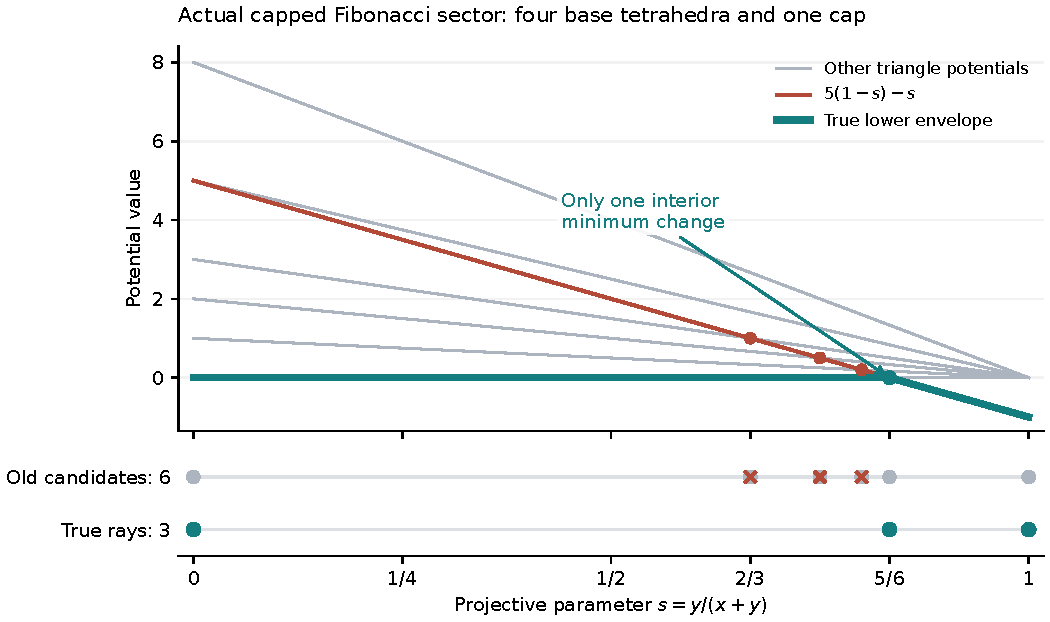
\includegraphics[width=\linewidth]{figures/minimum_envelope.pdf}
\caption{The actual potential functions for the capped family with $n=4$,
using the positive projective normalization $x+y=1$. Three interior
pairwise crossings fail to change the minimum and give no standard ray.
The true change at $s=5/6$, together with the endpoints, gives all three
rays. The lower strip marks the complete old candidate list and the exact
new output list.}
\label{fig:envelope}
\end{figure}

\begin{corollary}[Exact surplus in the old arrangement]
\label{cor:oldfamily}
For this family, the old arrangement has $n+3$ distinct projected hyperplanes,
$n+2$ nonzero nonnegative candidate directions, and $n-1$ nonextreme
directions that are rejected. The envelope method emits exactly three rays.
\end{corollary}

\begin{proof}
Modulo a common old-vertex potential, the distinct potential forms are
\[
 0,\ F_2x,\ F_3x,\ldots,F_{n+2}x,\ A_nx-y.
\]
The new vertex contributes no differences. Equalities between pure
multiples of $x$ all give $x=0$. The remaining equalities give
$y=(A_n-c)x$ for
$c\in\{0,F_2,F_3,\ldots,F_{n+2}\}$. There are $n+2$ distinct such
slopes, exactly one negative, arising from $c=B_n>A_n$. The quadrilateral
coordinate hyperplanes add none: $x=0$ already occurs and $y=0$ is the
case $c=A_n$. Thus there are $n+3$ distinct hyperplanes, of which $n+2$
give nonnegative directions. Theorem~\ref{thm:family} leaves only three
standard rays, so $n-1$ positive directions fail extremality. Their
intermediate equalities do not change the true minimum.
\end{proof}



For $n=1$, the three rows of the following table give the complete output.
The separating semicolon distinguishes triangles from quadrilaterals. The
second ray has an independently replayable disc certificate in
\texttt{examples/extra\_non\_q\_disc.json}.

\begin{table}[ht]
\centering\small
\begin{tabular}{@{}ccl@{}}
\toprule
$(x,y)$ & Original tetrahedron; cap tetrahedron & Topology\\
\midrule
$(1,0)$ & $(1,1,0,0;0,0,1)$; $(1,2,0,0;0,0,0)$ & Essential disc\\
$(1,1)$ & $(1,1,0,0;0,0,1)$; $(0,2,0,0;0,1,0)$ & Essential disc\\
$(0,1)$ & $(1,1,1,1;0,0,0)$; $(0,1,0,1;0,1,0)$ & Inessential disc\\
\bottomrule
\end{tabular}
\caption{The smallest capped-family sector. The interior standard ray is
absent from the quadrilateral vertex list.}
\end{table}

The formulas also give a direct family-specific oracle using $O(n)$
Fibonacci additions and coordinate operations. The complete output has
$\Theta(n^2)$ bits because it contains a linear sequence of Fibonacci
coordinates of linearly growing binary lengths. Standard binary addition
evaluates the formulas in $O(n^2)$ bit time. The delivered generic kernel
builder is not replaced by a special recognizer for this family; the formulas
serve as a separate mathematical description and are implemented as an oracle
in \texttt{experiments/family\_oracle.py}.
